\subsubsection{Logarithmen}
\begin{corollary}{Natürlicher Logarithmus}
   Der nat. Logarithmus $\ln:]0, + \infty[ \to \R$ ist eine streng monoton wachsende, stetige, bijektive Funktion. 
\end{corollary}
\begin{corollary}{Rechnen mit Logarithmen}
    \begin{enumerate}
        \item Für $a > 0$ ist $]0, \infty[ \to ]0 + \infty[$ \quad $x \mapsto x^a$ eine stetige, streng monoton wachsende Bijektion.
        \item Für $a < 0$ ist $]0, \infty[ \to ]0 + \infty[$ \quad $x \mapsto x^a$ eine stetige, streng monoton fallende Bijektion.
        \item $\ln (a \cdot b) = \ln a + \ln b \quad \forall a,b \in ]0 +  \infty[$
        \item $\ln (a \div b) = \ln a - \ln b \quad \forall a,b \in ]0 +  \infty[$
        \item ${\ln \left(x^a\right) = a \ln (x) \quad \forall a \in \R, \forall x > 0}$
        \item ${x^a \cdot x^b = x^{a+b} \quad a,b \in \R, \forall x > 0}$
        \item ${\left(x^a\right)^b = x^{a \cdot b} \quad \forall a,b \in \R, \forall x > 0}$
    \end{enumerate}
    Im Allgemeinen gilt: $log_b (a) = \frac{ln(a)}{ln(b)}$
\end{corollary}
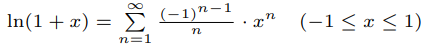
\includegraphics[scale=0.5]{Analysis1/zsf/Images/Basics/ln.png}
\subsubsection{Werte von log}
\begin{equation*}
	\begin{array}{lccccccc}
		& 0 & 1 & 2 & e & 3 & 5 & 10\\
		\ln & - \infty & 0 & 0.693 & 1 & 1.09 & 1.609 & 2.303\\
		\log_2 & - \infty & 0 & 1 & 1.443 & 1.585 & 2.321 & 3.321\\
		\log_{10} & - \infty & 0 & 0.301 & 0.434 & 0.477 & 0.699 & 1
	\end{array}
\end{equation*}
